%%%%%%%%%%%%%%%%%%%%%%%%%%ch3-1
\begin{frame}[shrink]
  \frametitle{ch3.信号检测与估计理论的基础知识}
  \framesubtitle{ch3-1. 统计检测理论基本概念及贝叶斯准则}
  \tableofcontents[hideallsubsections]
\end{frame}

\section{统计检测理论基本概念}

\begin{frame}{统计检测理论(假设检验理论)}
\begin{itemize}
	\item 统计信号处理的理论基础之一
	\item 主要研究在受噪声干扰的随机信号中,信号的有/无或信号属于哪个状态的最佳判决的概念、方法和性能等问题。
	\item 数学基础——统计判决理论,又称假设检验理论
\end{itemize}
\end{frame}

\begin{frame}{经典的信号统计检测理论}
\begin{itemize}
	\item 统计信号检测理论的基本概念
	\item 二元信号检测的最佳检测准则
	\item 信号状态的判决的方法和检测性能的分析
	\item M元信号的最佳检测
	\item 参量信号的复合假设检验
	\item 序列检测
\end{itemize}
\end{frame}

\section{二元信号检测}

\begin{frame}{统计检测理论的基本模型: 二元信号检测的模型}
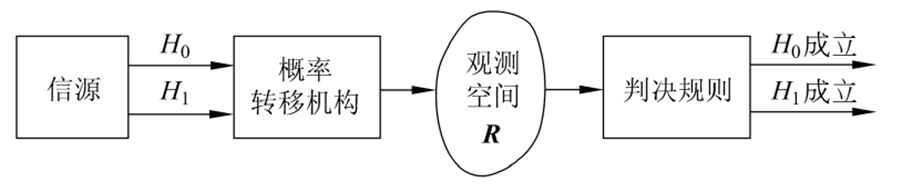
\includegraphics[scale=0.3]{model}
\begin{align*}
\textbf{信源}\implies &\text{\textcolor{blue}{信源的输出称为假设}}\\
\textbf{概率转移机构}\implies &\text{\textcolor{blue}{将信源的输出(假设)以一定的}}\\
&\text{\textcolor{blue}{概率关系映射到整个观察空间中}}\\
\textbf{观测空间}\implies &\text{\textcolor{blue}{接收端所有可能观测量的集合}}\\
\textbf{判决规则}\implies &\text{\textcolor{blue}{将观测空间进行合理划分, }}\\
&\text{\textcolor{blue}{使每个观测量对应一个假设判断的方法}}\\
\end{align*}
\end{frame}

\begin{frame}{统计检测理论的基本模型: 二元信号检测的模型示例1}
\begin{columns}
	\column{0.3\textwidth}
	\begin{align*}
	&H_1: r=1+n\\
	&H_0: r=-1+n\\
	&n:\text{噪声是一随机变量}\\
	&\text{一维观测空间:}\\
	&\bm{R}=\{-2,-1,0,1,2\}
	\end{align*}
	\column{0.7\textwidth}
	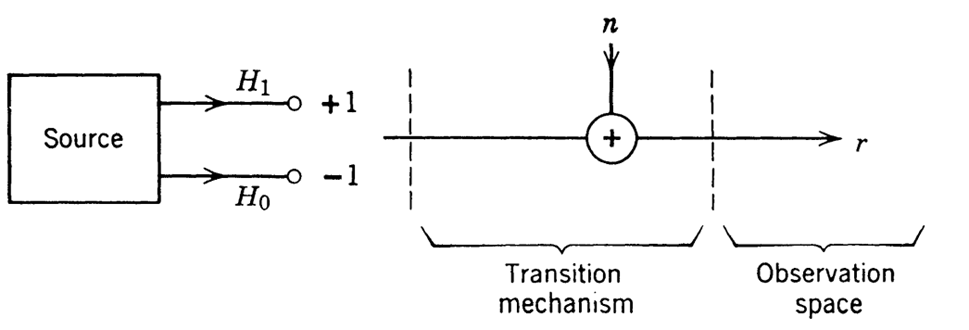
\includegraphics[scale=0.45]{ex-1m}\\
	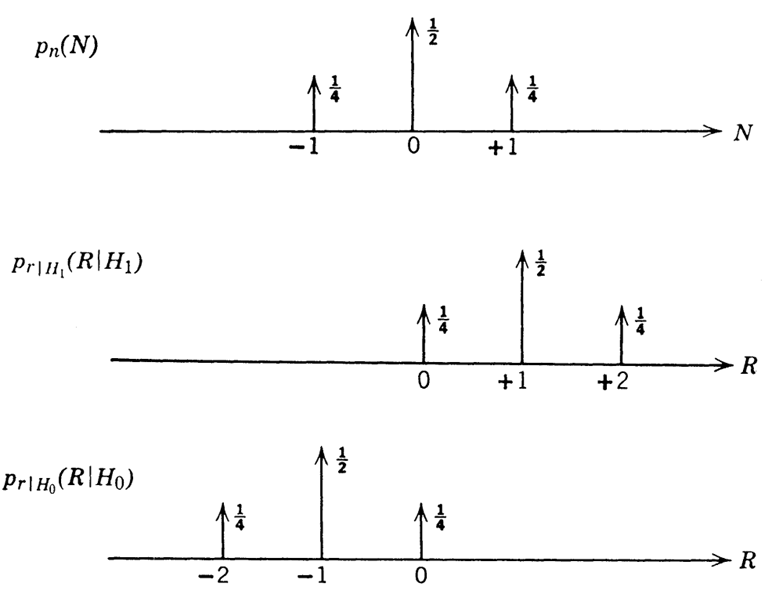
\includegraphics[scale=0.45]{ex-1}
\end{columns}
\end{frame}

\begin{frame}{统计检测理论的基本模型: 二元信号检测的模型示例2}
\begin{columns}
	\column{0.3\textwidth}
	\begin{align*}
	H_1: &r_1=1+n_1\\
	&r_2=1+n_2\\
	H_0: &r_1=-1+n_1\\
	&r_2=-1+n_2
	\end{align*}
	\begin{align*}
	&n_1,n_2:\text{噪声}\\
	&\text{二维观测空间:}\\
	&\bm{R}=\{R_1,R_2\}
	\end{align*}
	\column{0.7\textwidth}
	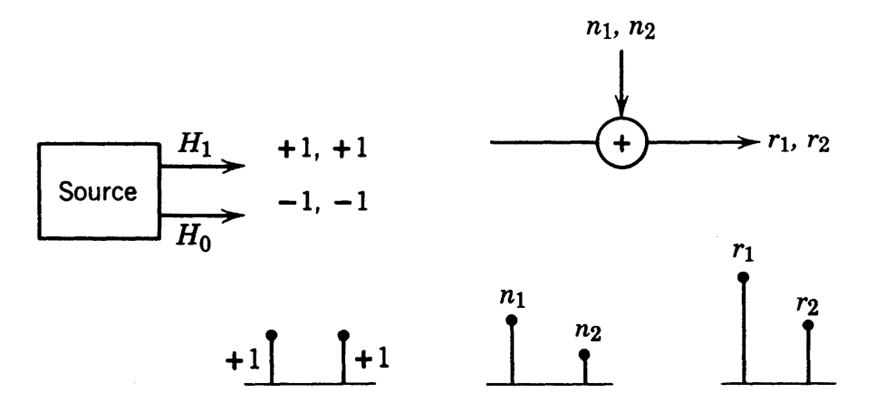
\includegraphics[scale=0.45]{ex-2m}\\
	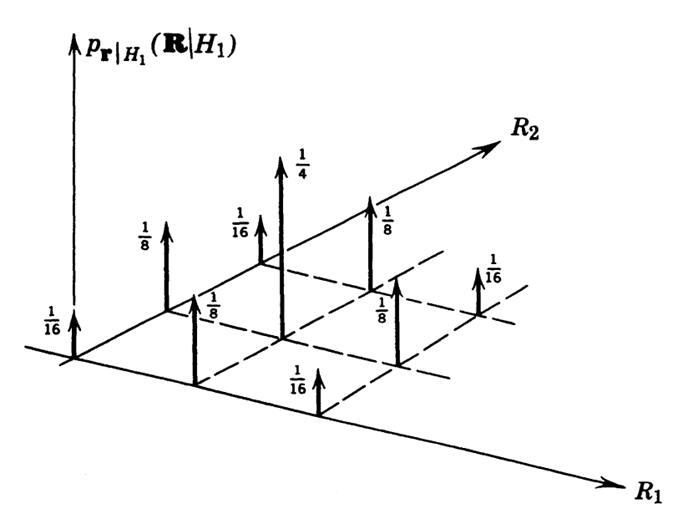
\includegraphics[scale=0.45]{ex-2}
\end{columns}
\end{frame}

\begin{frame}{统计检测理论的基本模型: 二元信号检测的判决域}
\begin{columns}
	\column{0.5\textwidth}
	二元信号的检测问题,可归结为\textcolor{blue}{\textbf{对观察空间的划分问题。}}\\
	即按照一定的准则,将观察空间$\bm{R}$分别划分为$R_0$和$R_1$两个子空间。\\
	\[\bm{R}=R_0\cup R_1,\quad R_0\cap R_1=\emptyset \]
	\column{0.5\textwidth}
	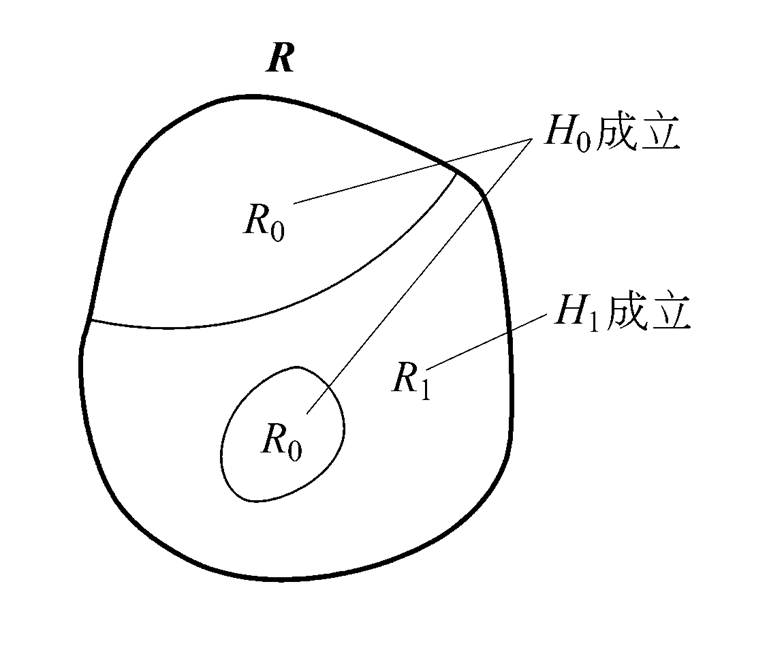
\includegraphics[scale=0.45]{R}\\
\end{columns}
\end{frame}

\begin{frame}
\begin{block}{思考}
	如果$n$是均值为零的, 方差为$\sigma_n^2$的高斯随机变量, 两个假设下的观测信号模型\\
	$H_1: r=1+n$\\
	$H_0: r=-1+n$\\
	观测信号$p(r|H_1),p(r|H_0)$应服从何种分布?
\end{block}
\end{frame}

\begin{frame}[shrink]
\begin{block}{思考}
	如果$n$是均值为零的, 方差为$\sigma_n^2$的高斯随机变量, 两个假设下的观测信号模型\\
	$H_1: r=1+n$\\
	$H_0: r=-1+n$\\
	观测信号$p(r|H_1),p(r|H_0)$应服从何种分布?
\end{block}
\begin{block}{}
	因为高斯随机变量的特点:高斯随机变量的线性组合还是高斯随机变量。\\
	习题2.7: $x\sim\mathcal{N}(\mu_x,\sigma_x^2)$,则$(y=ax+b)\sim\mathcal{N}(a\mu_x+b,a^2\sigma_x^2)$。\\
	所以, $p(r|H_1)\sim\mathcal{N}(1,\sigma_n^2)$, $p(r|H_0)\sim\mathcal{N}(-1,\sigma_n^2)$
\end{block}
\begin{block}{}
	$E(r|H_0)=E(1+n)=1+E(n)=1,$\\
	$Var(r|H_0)=E[(r|H_0-E(r|H_0))^2]=E[n^2]=\sigma_n^2\implies r|H_0\sim\mathcal{N}(1,\sigma_n^2)$\\
	$E(r|H_1)=E(-1+n)=-1+E(n)=-1,$\\
	$Var(r|H_1)=E[(r|H_1-E(r|H_1))^2]=E[n^2]=\sigma_n^2\implies r|H_1\sim\mathcal{N}(-1,\sigma_n^2)$
\end{block}
\end{frame}


\begin{frame}{统计检测理论的基本模型: 二元信号检测}
\textbf{考虑噪声$n$为高斯噪声时的概率转移机构}
\begin{columns}
	\column{0.45\textwidth}
	观测模型为:
	\begin{align*}
	H_0: x&=-A+n\\
	H_1: x&=A+n
	\end{align*}
	概率转移:\\
	信源输出的某一种确知信号:
	\begin{itemize}
		\item 无噪声干扰时,将映射到观测空间中的某一点;
		\item 有噪声干扰时,将以一定的概率映射到观测空间。而映射到某一点附件的概率决定于概率密度函数$p(x|H_j)(j=1,2)$.
	\end{itemize}
	\column{0.55\textwidth}
	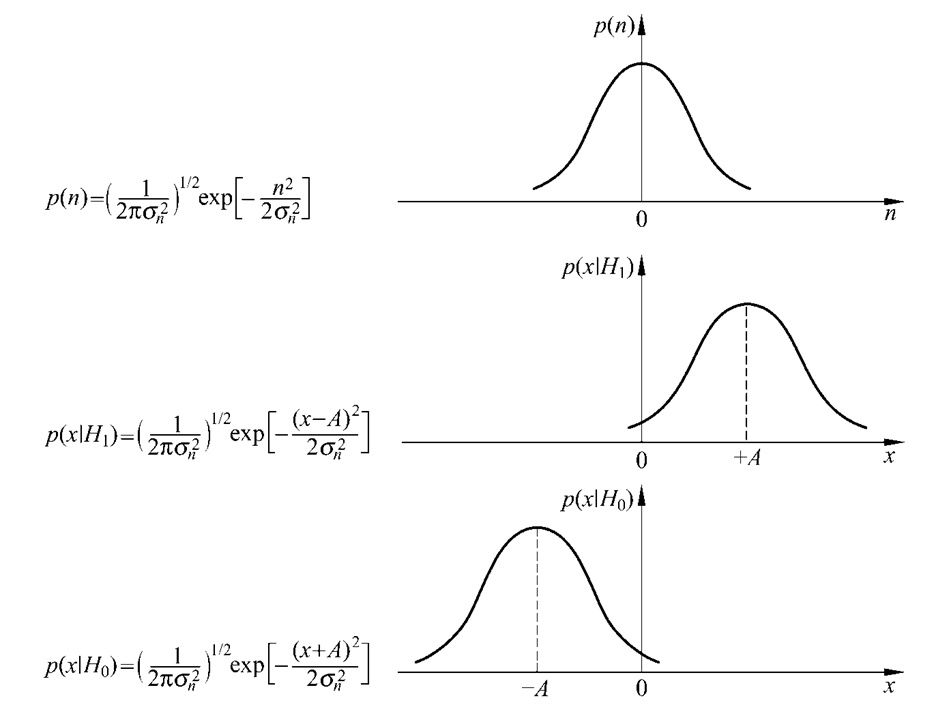
\includegraphics[scale=0.4]{model-n}
\end{columns}
\end{frame}

\section{M元信号检测}

\begin{frame}{统计检测理论的基本模型: M元信号检测}
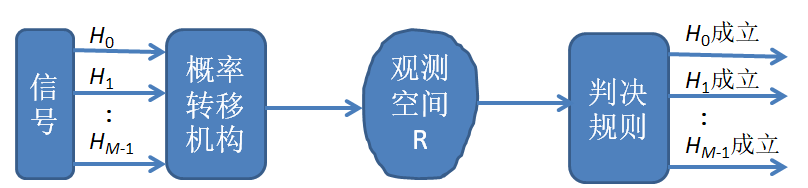
\includegraphics[scale=0.4]{M}
\newline
\begin{columns}
	\column{0.4\textwidth}
    判决域划分:
    \[\bm{R}=\bigcup_{i=0}^{M-1}R_i, R_i\cap R_j=\emptyset, (i\ne j) \]
	\column{0.6\textwidth}
	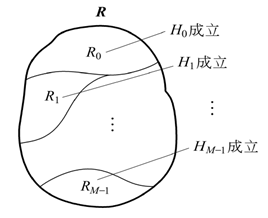
\includegraphics[scale=0.4]{R-M}
\end{columns}
\end{frame}

\section{判决结果和判决概率}

\begin{frame}{二元信号检测---统计检测判决结果和判决概率}
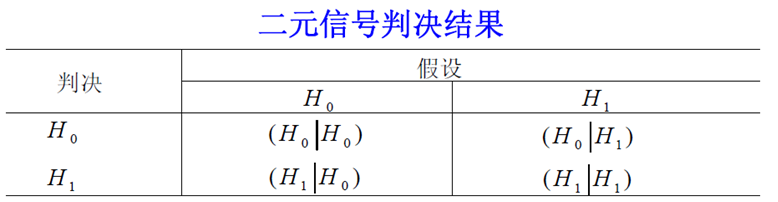
\includegraphics[scale=0.4]{2-result}\\
\textcolor{red}{$(H_i|H_j)(i,j=0,1)$: 在假设$H_j$为真的条件下,判决假设$H_i$成立的结果。}
\newline
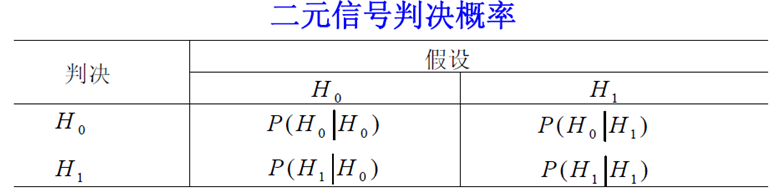
\includegraphics[scale=0.4]{2-P}\\
\textcolor{red}{$P(H_i|H_j)(i,j=0,1)$: 在假设$H_j$为真的条件下,判决假设$H_i$成立的概率。}
\end{frame}

\begin{frame}
\begin{columns}
	\column{0.5\textwidth}
	\begin{align*}
	&H_0: x=-A+n,\quad H_1: x=A+n\\
	&H_0: x_k=-A+n_k,\quad H_1: x_k=A+n_k\\
	&k=1,2,\dots,N,\quad \bm{x}=(x_1,x_2,\dots,x_N)^{T}\\
	&P(H_i|H_j)=\int_{R_i}p(\bm{x}|H_j)d\bm{x}
	\end{align*}
	\column{0.5\textwidth}
	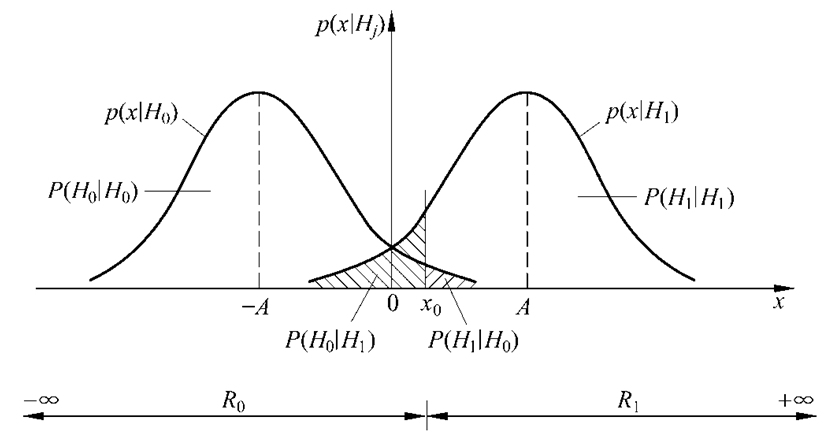
\includegraphics[scale=0.4]{detectionA}
\end{columns}
\begin{align*}
&P(H_0|H_0)=\int_{R_0}p(\bm{x}|H_0)d\bm{x},\qquad P(H_1|H_0)=\int_{R_1}p(\bm{x}|H_0)d\bm{x}\\
&P(H_0|H_1)=\int_{R_0}p(\bm{x}|H_1)d\bm{x},\qquad P(H_1|H_1)=\int_{R_1}p(\bm{x}|H_1)d\bm{x}\\
&\bm{R}=R_0\cup R_1,\quad R_0\cap R_1=\emptyset, \quad \int_{\bm{R}}p(\bm{x}|H_j)d\bm{x}=1\\
&P(H_0|H_0)+P(H_1|H_0)=\int_{R_0}p(\bm{x}|H_0)d\bm{x}+\int_{R_1}p(\bm{x}|H_0)d\bm{x}=\int_{\bm{R}}p(\bm{x}|H_0)d\bm{x}=1\\
&P(H_0|H_1)+P(H_1|H_1)=\int_{R_0}p(\bm{x}|H_1)d\bm{x}+\int_{R_1}p(\bm{x}|H_1)d\bm{x}=\int_{\bm{R}}p(\bm{x}|H_1)d\bm{x}=1
\end{align*}
\end{frame}

\section{判决域的划分}

\begin{frame}{信号统计检测理论要研究的基本问题---判决域的划分}
\begin{columns}
	\column{0.5\textwidth}
	\begin{align*}
	&H_0: x=-A+n,\quad H_1: x=A+n\\
	&H_0: x_k=-A+n_k,\quad H_1: x_k=A+n_k\\
	&k=1,2,\dots,N,\quad \bm{x}=(x_1,x_2,\dots,x_N)^{T}\\
	&P(H_i|H_j)=\int_{R_i}p(\bm{x}|H_j)d\bm{x}
	\end{align*}
	\column{0.5\textwidth}
	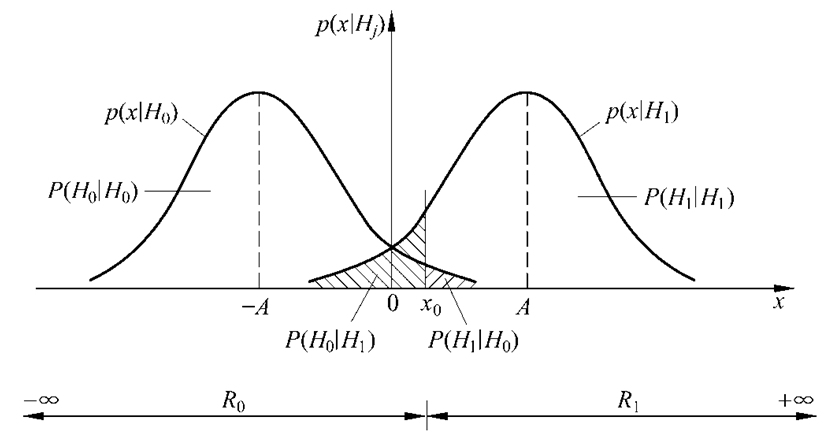
\includegraphics[scale=0.4]{detectionA}
\end{columns}
\begin{itemize}
	\item 目标: 正确判决概率$P(H_j|H_j)$尽可能大,错误判决概率$P(H_i|H_j)(i\ne j)$尽可能小。
	\item $x_0\downarrow\implies$正确判决概率$P(H_1|H_1)\uparrow$, 但另一个正确判决概率$P(H_0|H_0)\downarrow$。
	\item $x_0\downarrow\implies$错误判决概率$P(H_0|H_1)\downarrow$, 但另一个错误判决概率$P(H_1|H_0)\uparrow$。
	\item $x_0\uparrow\implies$正确判决概率$P(H_0|H_0)\uparrow$, 但另一个正确判决概率$P(H_1|H_1)\downarrow$。
	\item $x_0\uparrow\implies$错误判决概率$P(H_1|H_0)\downarrow$, 但另一个错误判决概率$P(H_0|H_1)\uparrow$。
	\item 判决域的划分影响判决概率$P(H_i|H_j)$, 因此需要最佳划分判决域。
\end{itemize}
\end{frame}

\begin{frame}{信号统计检测理论要研究的基本问题---判决域的划分}
\begin{columns}
	\column{0.5\textwidth}
	\begin{align*}
	&H_0: x=-A+n,\quad H_1: x=A+n\\
	&H_0: x_k=-A+n_k,\quad H_1: x_k=A+n_k\\
	&k=1,2,\dots,N,\quad \bm{x}=(x_1,x_2,\dots,x_N)^{T}\\
	&P(H_i|H_j)=\int_{R_i}p(\bm{x}|H_j)d\bm{x}
	\end{align*}
	\column{0.5\textwidth}
	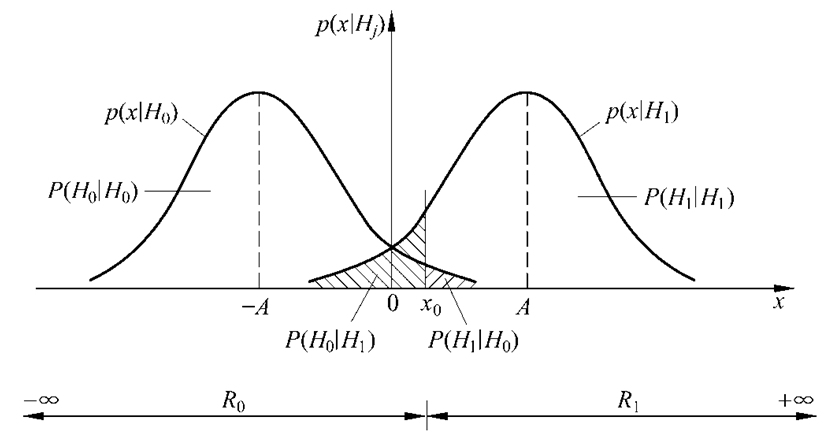
\includegraphics[scale=0.4]{detectionA}
\end{columns}
\begin{itemize}
	\item 目标: 正确判决概率$P(H_j|H_j)$尽可能大,错误判决概率$P(H_i|H_j)(i\ne j)$尽可能小。
	\item 判决域的划分影响判决概率$P(H_i|H_j)$, 因此需要最佳划分判决域。
	\item $p(\bm{x}|H_j)(j=0,1)$: 假设$H_j$下观测信号的概率密度函数。它描述观测(接收)信号的统计特性。
	\item 按照一定的准则,将观测空间$\bm{R}$分别划分为$R_0$和$R_1$两个子空间。
	计算判决概率$P(H_i|H_j)(i,j=0,1)$。	
\end{itemize}
\end{frame}

\begin{frame}{二元信号检测---统计检测判决结果和判决概率计算}
	\textbf{观测模型为:}
	\begin{align*}
	H_0: x&=n\\
	H_1: x&=A+n
	\end{align*}
	\textbf{考虑噪声$n$是均值为零, 方差为$\sigma^2$的高斯噪声, 且不同时刻的加性噪声之间是相互统计独立的。}\\
	\textcolor{blue}{\textbf{接收端根据接收信号判决时,会出现四种事件,对应四个判决概率:}}\\
	\centering
	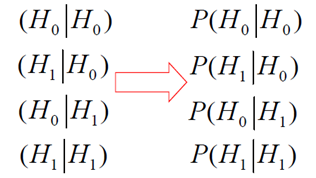
\includegraphics[scale=0.4]{HH}
\end{frame}

\begin{frame}{二元信号检测---统计检测判决结果和判决概率计算}
\begin{columns}
	\column{0.5\textwidth}
	\textbf{观测模型为:}
	\begin{align*}
	&H_0: x=-A+n\\
	&H_1: x=A+n
	\end{align*}
	\textbf{考虑噪声$n\sim\mathcal{N}(0,\sigma^2)$, 且不同时刻的加性噪声之间是相互统计独立的。}\\
	\column{0.5\textwidth}
	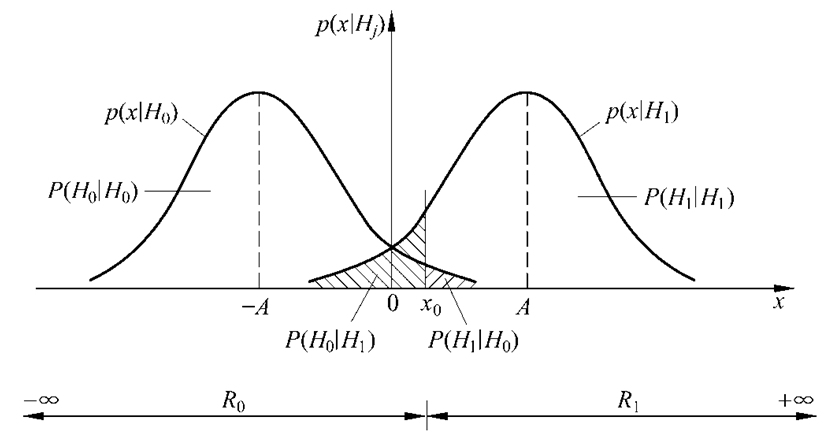
\includegraphics[scale=0.4]{detectionA}
\end{columns}
\[ \text{噪声$n$的概率密度: \qquad} p(n)=\left(\frac{1}{2\pi\sigma^2}\right)^{1/2}\exp\left(-\frac{n^2}{2\sigma^2}\right)\]
接收信号$\bm{x}$的统计特性可以描述为:
\begin{align*}
p(\bm{x}|H_0)&=\left(\frac{1}{2\pi\sigma^2}\right)^{1/2}\exp\left[-\frac{(x+A)^2}{2\sigma^2}\right]\\
p(\bm{x}|H_1)&=\left(\frac{1}{2\pi\sigma^2}\right)^{1/2}\exp\left[-\frac{(x-A)^2}{2\sigma^2}\right]
\end{align*}
\end{frame}

\begin{frame}[shrink]{二元信号检测---统计检测判决结果和判决概率计算}
\begin{columns}
	\column{0.5\textwidth}
	\textbf{观测模型为:}
	\begin{align*}
	&H_0: x=-A+n\\
	&H_1: x=A+n
	\end{align*}
	\textbf{考虑噪声$n\sim\mathcal{N}(0,\sigma^2)$, 且不同时刻的加性噪声之间是相互统计独立的。}\\
	\column{0.5\textwidth}
	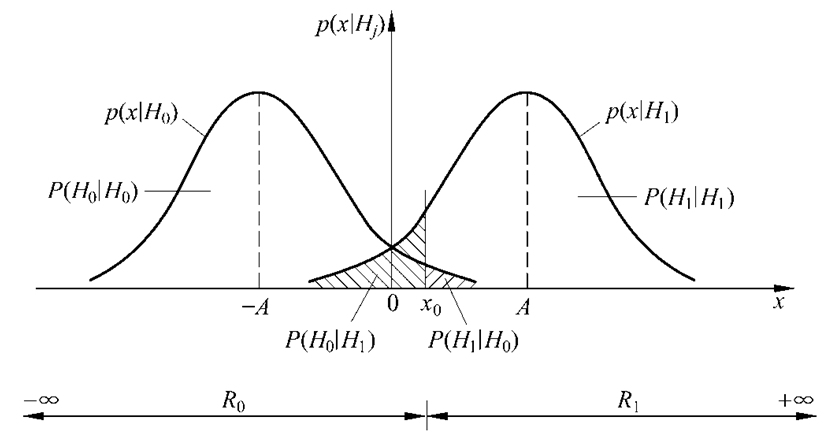
\includegraphics[scale=0.4]{detectionA}
\end{columns}
\[\text{四种判决概率的计算:}\quad P(H_i|H_j)=\int_{R_i}p(\bm{x}|H_j)d\bm{x} \]
\begin{align*}
&P(H_0|H_0)=\int_{R_0}p(\bm{x}|H_0)d\bm{x},\qquad P(H_1|H_0)=\int_{R_1}p(\bm{x}|H_0)d\bm{x}\\
&P(H_0|H_1)=\int_{R_0}p(\bm{x}|H_1)d\bm{x},\qquad P(H_1|H_1)=\int_{R_1}p(\bm{x}|H_1)d\bm{x}\\
&\bm{R}=R_0\cup R_1,\quad R_0\cap R_1=\emptyset, \quad \int_{\bm{R}}p(\bm{x}|H_j)d\bm{x}=1\\
&P(H_0|H_0)+P(H_1|H_0)=\int_{R_0}p(\bm{x}|H_0)d\bm{x}+\int_{R_1}p(\bm{x}|H_0)d\bm{x}=\int_{\bm{R}}p(\bm{x}|H_0)d\bm{x}=1\\
&P(H_0|H_1)+P(H_1|H_1)=\int_{R_0}p(\bm{x}|H_1)d\bm{x}+\int_{R_1}p(\bm{x}|H_1)d\bm{x}=\int_{\bm{R}}p(\bm{x}|H_1)d\bm{x}=1
\end{align*}
\end{frame}

\begin{frame}{术语}
\textcolor{blue}{$H_j(j=0,1)$: 信源输出的信号, 称为假设$H_j$}

\bigskip

\textcolor{blue}{$P(H_j)(i=0)$: 假设$H_j$为真的先验概率(先验:先于试验)}


\bigskip
\textcolor{blue}{$(x|H_j)(j=0,1)$: 假设$H_j$下的观测信号是随机变量}

\bigskip

\textcolor{blue}{$p(x|H_j)(j=0,1)$: 假设$H_j$下观测信号的概率密度函数}

\bigskip

\textcolor{blue}{$(H_i|H_j)(i,j=0,1)$: 在假设$H_j$为真的条件下,判决假设$H_i$成立的结果。}\\
~\\
\textcolor{blue}{$P(H_i|H_j)(i,j=0,1)$: 在假设$H_j$为真的条件下,判决假设$H_i$成立的概率。}\\
\end{frame}

\section{贝叶斯准则}

\begin{frame}{贝叶斯准则---基本要求}
\begin{itemize}
	\item 充分理解平均代价(Average risk)的概念
	\item 贝叶斯准则(Bayes criterion)的判决表达式
	\item 判决性能分析
\end{itemize}

\bigskip
\textcolor{blue}{贝叶斯准则的基本原理:在划分观察空间时,使平均代价最小。}
\end{frame}

\begin{frame}{信号统计检测理论要研究的基本问题---判决域的划分}
\begin{columns}
	\column{0.5\textwidth}
	\begin{align*}
	&H_0: x=-A+n,\quad H_1: x=A+n\\
	&H_0: x_k=-A+n_k,\quad H_1: x_k=A+n_k\\
	&k=1,2,\dots,N,\quad \bm{x}=(x_1,x_2,\dots,x_N)^{T}\\
	&P(H_i|H_j)=\int_{R_i}p(\bm{x}|H_j)d\bm{x}
	\end{align*}
	\column{0.5\textwidth}
	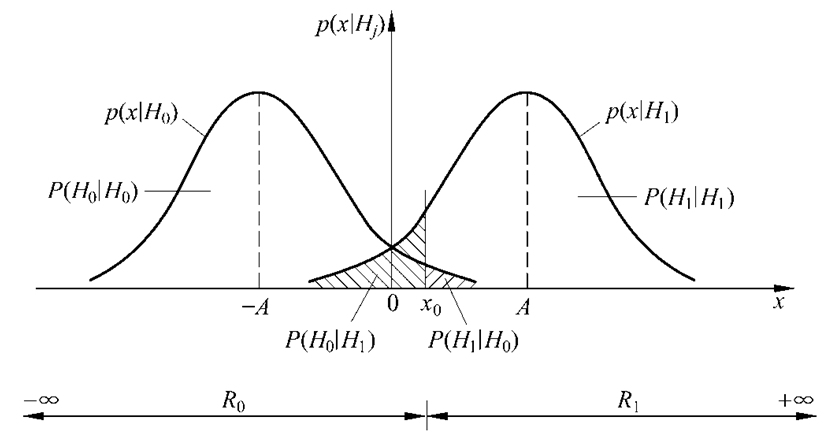
\includegraphics[scale=0.4]{detectionA}
\end{columns}
\begin{itemize}
	\item 目标: 正确判决概率$P(H_j|H_j)$尽可能大,错误判决概率$P(H_i|H_j)(i\ne j)$尽可能小。
	\item 判决域的划分影响判决概率$P(H_i|H_j)$, 因此\textbf{需要最佳划分判决域}。
	\item $p(\bm{x}|H_j)(j=0,1)$: 假设$H_j$下观测信号的概率密度函数。它描述观测(接收)信号的统计特性。
	\item 按照一定的准则,将观察空间$\bm{R}$分别划分为$R_0$和$R_1$两个子空间。
	计算判决概率$P(H_i|H_j)(i,j=0,1)$。	
\end{itemize}
\end{frame}

\begin{frame}{贝叶斯检测的提出动机}
通信系统中, 二元信号的平均解调错误概率(由全概率公式得出):
\[ P_e=P(0)P(1|0)+P(1)P(0|1)\]
可以看出, 检测性能不仅与两种错误判决概率$[P(1|0),P(0|1)]$有关, 还与信源发送的0和1的先验概率$[P(0),P(1)]$有关。\\
另外, 每做出一种判断, 人们要付出的代价也是不同的。\\
如何综合考虑上述因素来设计好的检测方法?
\begin{block}{贝叶斯检测}
	给定各种判决代价因子, 且已知各假设的先验概率条件下,使\textbf{平均代价最小}的检测准则。
\end{block}
\end{frame}

\begin{frame}{问题}
\begin{enumerate}
	\item 代价因子如何定义?
	\item 平均代价如何计算?
	\item 如何获得最小的平均代价?
\end{enumerate}
\end{frame}

\begin{frame}{代价因子的定义}
\begin{block}{对于二元信号统计检测, 共有四种事件发生, 即}
$$
\begin{array}{cccc}
	(H_0|H_0) & (H_1|H_0) & (H_1|H_1) & (H_0|H_1)\\
	\Downarrow & \Downarrow & \Downarrow & \Downarrow\\
	c_{00} & c_{10} & c_{11} & c_{01}
\end{array}
$$
$c_{ij}$表示假设$H_j$为真时, 判决假设$H_i$成立所付出的代价
\end{block}
\begin{block}{Notes}
	一般地, $c_{10}>c_{00}, c_{01}>c_{11}$
\end{block}
\end{frame}

\begin{frame}{平均代价的计算}
\begin{block}{平均代价$C$由两部分构成}
	\begin{enumerate}
		\item 信源发送$H_0$假设时, 判决所付出的代价$C(H_0)$
		\item 信源发送$H_1$假设时, 判决所付出的代价$C(H_0)$
	\end{enumerate}
    \[C=P(H_0)C(H_0)+P(H_1)C(H_1)\]
\end{block}
参见:
\[ P_e=P(0)P(1|0)+P(1)P(0|1)\]
\end{frame}

\begin{frame}{平均代价的计算}
\begin{block}{对于二元信号统计检测, 共有四种事件发生, 即}
	$$
	\begin{array}{cccc}
	(H_0|H_0) & (H_1|H_0) & (H_1|H_1) & (H_0|H_1)\\
	\Downarrow & \Downarrow & \Downarrow & \Downarrow\\
	c_{00} & c_{10} & c_{11} & c_{01}
	\end{array}
	$$
	$c_{ij}$表示假设$H_j$为真时, 判决假设$H_i$成立所付出的代价
\end{block}
\begin{block}{因此, 两种假设下, 判决所付出的代价: }
   \begin{align*}
   C(H_0)&=c_{00}P(H_0|H_0)+c_{10}P(H_1|H_0)\\
   C(H_1)&=c_{01}P(H_0|H_1)+c_{11}P(H_1|H_1)
   \end{align*}
\end{block}
 平均代价: $C=P(H_0)C(H_0)+P(H_1)C(H_1)$
\end{frame}

\begin{frame}{平均代价的计算}
\begin{align*}
C&=P(H_0)C(H_0)+P(H_1)C(H_1)\\
C(H_0)&=c_{00}P(H_0|H_0)+c_{10}P(H_1|H_0)\\
C(H_1)&=c_{01}P(H_0|H_1)+c_{11}P(H_1|H_1)
\end{align*}
\centering $\Downarrow$
\begin{align*}
C=&P(H_0)c_{00}P(H_0|H_0)+c_{10}P(H_1|H_0)+\\
&P(H_1)c_{01}P(H_0|H_1)+c_{11}P(H_1|H_1)
\end{align*}
\end{frame}

\begin{frame}[shrink]{平均代价的计算}
\begin{columns}
	\column{0.55\textwidth}
	\begin{align*}
	C=&P(H_0)c_{00}P(H_0|H_0)+c_{10}P(H_1|H_0)+\\
	&P(H_1)c_{01}P(H_0|H_1)+c_{11}P(H_1|H_1)
	\end{align*}
	\[ P(H_i|H_j)=\int_{R_i}p(x|H_j)dx\]
	\column{0.35\textwidth}
	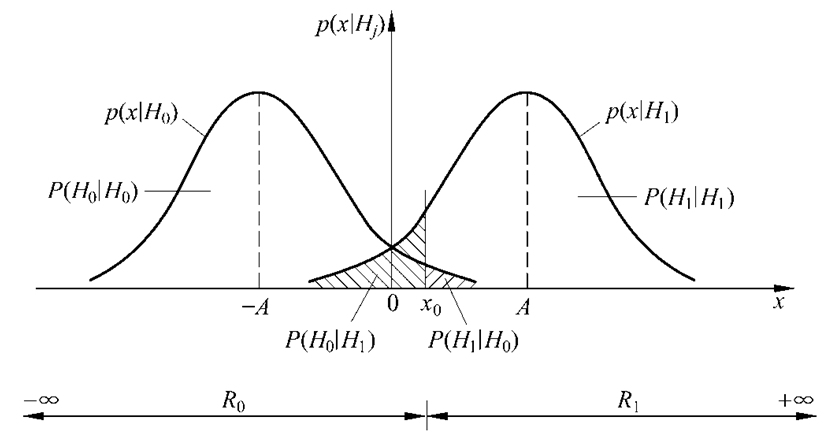
\includegraphics[scale=0.35]{detectionA}
\end{columns}

\medskip
\centering $\Downarrow$
\begin{align*}
C=&P(H_0)\left(c_{00}\int_{R_0}p(x|H_0)dx+c_{10}\int_{R_1}p(x|H_0)dx\right)+\\
&P(H_1)\left(c_{01}\int_{R_0}p(x|H_1)dx+c_{11}\int_{R_1}p(x|H_1)dx\right)
\end{align*}

\end{frame}

\begin{frame}[shrink]{平均代价的计算}
\begin{columns}
	\column{0.7\textwidth}
	\begin{align*}
	C=&P(H_0)\left(c_{00}\int_{R_0}p(x|H_0)dx+c_{10}\int_{R_1}p(x|H_0)dx\right)+\\
	&P(H_1)\left(c_{01}\int_{R_0}p(x|H_1)dx+c_{11}\int_{R_1}p(x|H_1)dx\right)
	\end{align*}
	\[\int_{R}p(x|H_j)dx=1 \implies \int_{R_1}p(x|H_j)dx=1-\int_{R_0}p(x|H_0)dx \]
	\column{0.3\textwidth}
	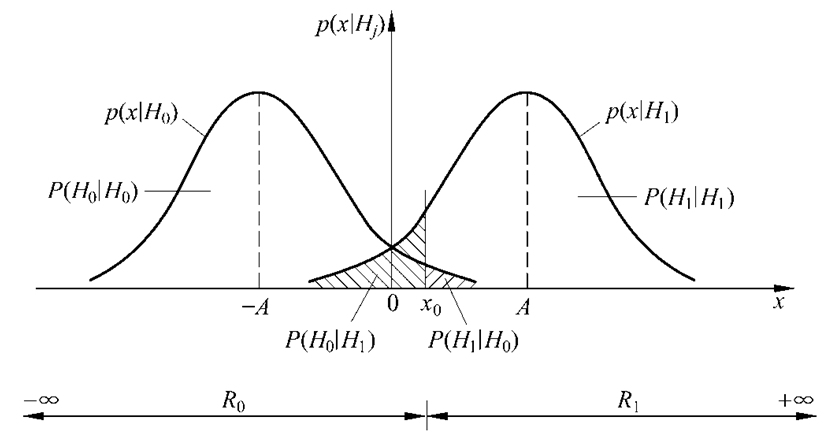
\includegraphics[scale=0.27]{detectionA}
\end{columns}

\medskip
\centering $\Downarrow$
\begin{align*}
C=&P(H_0)\left(c_{00}\int_{R_0}p(x|H_0)dx+c_{10}\left(1-\int_{R_0}p(x|H_0)dx\right)\right)+\\
&P(H_1)\left(c_{01}\int_{R_0}p(x|H_1)dx+c_{11}\left(1-\int_{R_0}p(x|H_1)dx\right)\right)
\end{align*}
\end{frame}

\begin{frame}[shrink]{平均代价的计算}
\begin{align*}
C=&P(H_0)\left(c_{00}\int_{R_0}p(x|H_0)dx+c_{10}\left(1-\int_{R_0}p(x|H_0)dx\right)\right)+\\
&P(H_1)\left(c_{01}\int_{R_0}p(x|H_1)dx+c_{11}\left(1-\int_{R_0}p(x|H_1)dx\right)\right)\\
=&P(H_0)\left(c_{10}+c_{00}\int_{R_0}p(x|H_0)dx-c_{10}\int_{R_0}p(x|H_0)dx\right)+\\
&P(H_1)\left(c_{11}+c_{01}\int_{R_0}p(x|H_1)dx-c_{11}\int_{R_0}p(x|H_1)dx\right)\\
=&c_{10}P(H_0)+c_{11}P(H_1)+\\
&\left(\int_{R_0}\left[P({H_1})(c_{01}-c_{11})p(x|H_1)-P(H_0)(c_{10}-c_{00})p(x|H_0)\right]dx \right)
\end{align*}
\end{frame}

\begin{frame}[shrink]{平均代价取最小的条件}
\begin{align*}
C=&c_{10}P(H_0)+c_{11}P(H_1)+\\
&\left(\int_{R_0}\left[P({H_1})(c_{01}-c_{11})p(x|H_1)-P(H_0)(c_{10}-c_{00})p(x|H_0)\right]dx \right)
\end{align*}
\begin{columns}
	\column{0.46\textwidth}
	$c_{10}P(H_0)$和$c_{11}P(H_1$是两项固定的值\\
	$P({H_1})(c_{01}-c_{11})p(x|H_1)\ge 0$\\
	$P(H_0)(c_{10}-c_{00})p(x|H_0)\ge 0$
	\column{0.35\textwidth}
	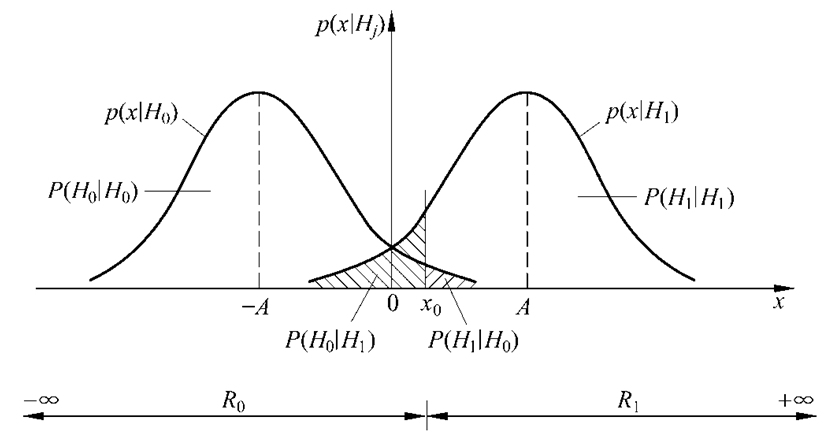
\includegraphics[scale=0.35]{detectionA}
\end{columns}
\begin{itemize}
	\item \textcolor{blue}{\textbf{因此, 给定信道特性和先验信息, 平均代价$C$的大小完全由判决域$R_0$确定。}}
	\item \textbf{把被积函数取负值的观测值$x$划分给$R_0$区域, 而把其余的观测值$x$划分给$R_1$, 即可保证平均代价最小。}
\end{itemize}
\end{frame}

\begin{frame}[shrink]{平均代价取最小的条件}
\begin{align*}
C=&c_{10}P(H_0)+c_{11}P(H_1)+\\
&\left(\int_{R_0}\left[P({H_1})(c_{01}-c_{11})p(x|H_1)-P(H_0)(c_{10}-c_{00})p(x|H_0)\right]dx \right)
\end{align*}
\begin{columns}
	\column{0.46\textwidth}
	\textbf{把被积函数取负值的观测值$x$划分给$R_0$区域, 而把其余的观测值$x$划分给$R_1$, 即可保证平均代价最小。}
	\column{0.35\textwidth}
	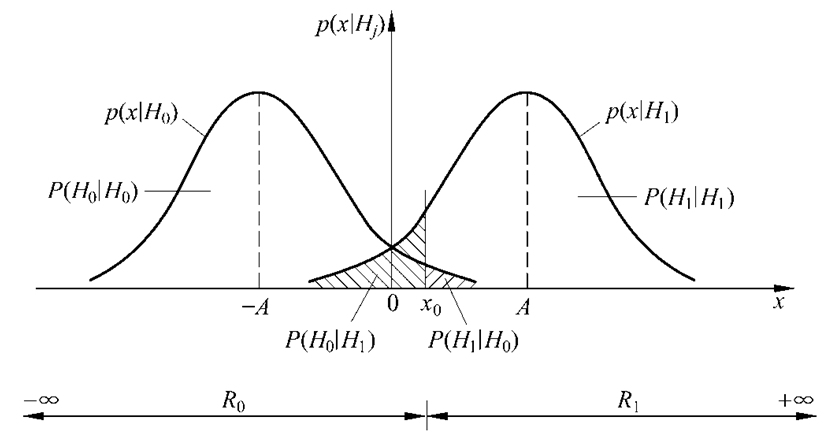
\includegraphics[scale=0.35]{detectionA}
\end{columns}
\begin{align*}
&P({H_1})(c_{01}-c_{11})p(x|H_1)< P(H_0)(c_{10}-c_{00})p(x|H_0)&\textbf{判决$H_0$假设成立}\\
&P({H_1})(c_{01}-c_{11})p(x|H_1)\ge P(H_0)(c_{10}-c_{00})p(x|H_0)&\textbf{判决$H_1$假设成立}
\end{align*}
\end{frame}

\begin{frame}{解决方案}
\begin{enumerate}
	\item 代价因子如何定义? \\
	$c_{ij}$表示假设$H_j$为真时, 判决假设$H_i$成立所付出的代价。\\
	$c_{00}, c_{10}, c_{11}, c_{01}$
	\item 平均代价如何计算?
	\begin{align*}
	C=&P(H_0)C(H_0)+P(H_1)C(H_1)\\
	&c_{10}P(H_0)+c_{11}P(H_1)+\\
	&\left(\int_{R_0}\left[P({H_1})(c_{01}-c_{11})p(x|H_1)-P(H_0)(c_{10}-c_{00})p(x|H_0)\right]dx \right)
	\end{align*}
	\item 如何获得最小的平均代价?
	\begin{align*}
	&P({H_1})(c_{01}-c_{11})p(x|H_1)< P(H_0)(c_{10}-c_{00})p(x|H_0)&\textbf{判决$H_0$假设成立}\\
	&P({H_1})(c_{01}-c_{11})p(x|H_1)\ge P(H_0)(c_{10}-c_{00})p(x|H_0)&\textbf{判决$H_1$假设成立}
	\end{align*}
\end{enumerate}
\end{frame}

\begin{frame}[shrink]{贝叶斯判决准则}
\begin{columns}%[t]
	\column{0.25\textwidth}
	\textbf{二元信号检测模型:}
	\column{0.2\textwidth}
	\begin{align*}
	H_0: &x=-A+n\\
	H_1: &x=A+n
	\end{align*}
	\column{0.35\textwidth}
	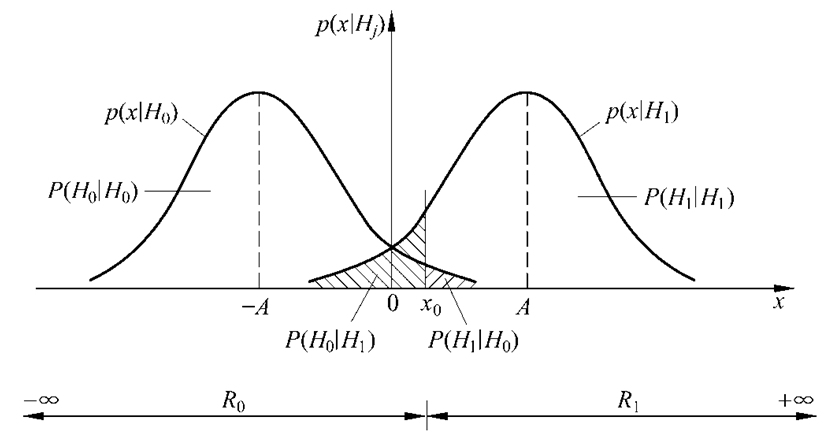
\includegraphics[scale=0.3]{detectionA}
\end{columns}
\begin{align*}
&P({H_1})(c_{01}-c_{11})p(x|H_1)< P(H_0)(c_{10}-c_{00})p(x|H_0)&\textbf{判决$H_0$假设成立}\\
&P({H_1})(c_{01}-c_{11})p(x|H_1)\ge P(H_0)(c_{10}-c_{00})p(x|H_0)&\textbf{判决$H_1$假设成立}
\end{align*}
\begin{block}{贝叶斯判决准则}
	\begin{align*}
	\frac{p(x|H_1)}{p(x|H_0)}&<\frac{P(H_0)(c_{10}-c_{00})}{P(H_1)(c_{01}-c_{11})}&\textbf{判决$H_0$假设成立}\\
	\frac{p(x|H_1)}{p(x|H_0)}&\ge\frac{P(H_0)(c_{10}-c_{00})}{P(H_1)(c_{01}-c_{11})}&\textbf{判决$H_1$假设成立}
	\end{align*}
\end{block}
\end{frame}

\begin{frame}{贝叶斯判决准则}
\begin{block}{贝叶斯判决准则}
	\begin{align*}
	\frac{p(x|H_1)}{p(x|H_0)}&<\frac{P(H_0)(c_{10}-c_{00})}{P(H_1)(c_{01}-c_{11})}&\textbf{判决$H_0$假设成立}\\
	\frac{p(x|H_1)}{p(x|H_0)}&\ge\frac{P(H_0)(c_{10}-c_{00})}{P(H_1)(c_{01}-c_{11})}&\textbf{判决$H_1$假设成立}
	\end{align*}
	$\implies$
	\[ \frac{p(x|H_1)}{p(x|H_0)}\mathop{\gtrless}_{H_0}^{H_1}\frac{P(H_0)(c_{10}-c_{00})}{P(H_1)(c_{01}-c_{11})} \]
	$\implies$
	\[\lambda(x)\mathop{\gtrless}_{H_0}^{H_1}\eta \]
\end{block}
\end{frame}

\begin{frame}{贝叶斯判决准则}
\begin{block}{贝叶斯判决准则}
	\[ \frac{p(x|H_1)}{p(x|H_0)}\mathop{\gtrless}_{H_0}^{H_1}\frac{P(H_0)(c_{10}-c_{00})}{P(H_1)(c_{01}-c_{11})} \implies \lambda(x)\mathop{\gtrless}_{H_0}^{H_1}\eta \]
	\begin{align*}
	&\lambda(x)\mathop{=}\limits^{def}\frac{p(x|H_1)}{p(x|H_0)} &&\textbf{定义为}\textcolor{blue}{\textbf{似然比函数}}\\
	&\eta\mathop{=}\limits^{def}\frac{P(H_0)(c_{10}-c_{00})}{P(H_1)(c_{01}-c_{11})} &&\textbf{定义为}\textcolor{blue}{定义为\textbf{判决门限}}
	\end{align*}
\end{block}
\textbf{$\lambda(x)$是一维随机变量, 称为\textcolor{blue}{检验统计量}}\\
\textbf{$\lambda(x)$不依赖于假设的先验概率$[P(H_0), P(H_1)]$, 也与代价因子无关。\textcolor{blue}{适用于不同先验概率和不同代价因子的最佳信号检测。}}
\end{frame}

\begin{frame}[shrink]
\frametitle{ch3.信号检测与估计理论的基础知识}
\framesubtitle{ch3-1. 统计检测理论基本概念及贝叶斯准则}
\tableofcontents[hideallsubsections]
\end{frame}



